\documentclass[10pt,a4paper]{article}
\usepackage[utf8]{inputenc}
\usepackage[left=2cm,right=2cm,top=2cm,bottom=2cm]{geometry}
\usepackage[colorlinks,linkcolor=blue,citecolor=blue,urlcolor=blue]{hyperref}
\usepackage{titlesec}
\usepackage{enumitem}
\usepackage{fancyhdr}
\usepackage{subcaption}
\usepackage{../preamble_math}
\usepackage{cleveref}

\newtheorem{exercici}{Exercice}
\theoremstyle{remark}
\newtheorem*{res}{Resolution}

\titleformat{\section}
  {\normalfont\fontsize{11}{15}\bfseries}{\thesection}{1em}{}

% \renewcommand{\theenumi}{\textbf{\arabic{enumi}}}
\renewcommand{\theenumi}{\alph{enumi}}
\renewcommand{\theenumiii}{\roman{enumiii}}
\setlength\multlinegap{0pt} % disable the margins on \begin{multline} command.

\title{\bfseries\Large Tutorial 2}

\author{Víctor Ballester Ribó}
\date{\parbox{\linewidth}{\centering
  Turbulence\endgraf
  M2 Applied and Theoretical Mathematics\endgraf
  Université Paris-Dauphine\endgraf
  Februrary 2024\endgraf}}
  %\setlength{\headheight}{13.6pt}

\setlength{\parindent}{0pt}
\begin{document}
\maketitle
\begin{exercici}\label{ex:1}
  In this homework, we will explore some properties of Burgers equation.
  \begin{align}
    \partial_t V_i + V_j \partial_j V_i & = \nu \laplacian V_i,\label{eq:11} \\
    V_i                                 & = -\partial_i \Psi,\label{eq:12}
  \end{align}
  \begin{enumerate}
    \item Use equation \eqref{eq:12} to find the equation for $\Psi$.
    \item 1D case: Check that the ``Khokhlov'' velocity field $u^\nu(x,t) = (x - L \tanh(Lx/(2\nu t)))/t$ is a solution of Burgers equation \eqref{eq:11}. Draw it at several times for $L = 1$, and $\nu = 1, \nu = 10^{-2}$ and $\nu = 10^{-6}$.
    \item Find the limit of the Khokhlov solution when $\nu \to 0$. This solution represents a shock.
  \end{enumerate}
\end{exercici}
\begin{res}\hfill
  \begin{enumerate}
    \item Putting \eqref{eq:12} into \eqref{eq:11} we get:
          \begin{align}
            \nonumber-\partial_t \partial_i \Psi + \partial_j \Psi\partial_j \partial_i \Psi  & = -\nu \partial_j^2 \partial_i \Psi \\
            \nonumber\partial_i\left( \partial_t \Psi - \frac{1}{2}(\partial_j \Psi)^2\right) & = \partial_i (\nu \laplacian  \Psi) \\
            \label{eq:psi} \partial_t \Psi - \frac{1}{2}(\partial_j \Psi)^2                   & = \nu \laplacian  \Psi + f(t)
          \end{align}
          Note that the constant $f(t)$ does not depend on any spatial variable $i$, because for each $i$, we have the same equation for $\Psi$. Thus, it can only depend on time.
    \item We need to check that:
          \begin{equation*}
            \partial_t u^\nu + u^\nu \partial_x u^\nu = \nu \partial_{xx} u^\nu
          \end{equation*}
          We have that:
          \begin{align*}
            \partial_t u^\nu        & =- \frac{ \left(x-L\tanh\left(\frac{Lx}{2\nu t}\right)\right)}{t^2} + \frac{L^2x}{2\nu t^3} \sech^2\left(\frac{Lx}{2\nu t}\right)                                                                                                   \\
            \partial_x u^\nu        & = \frac{1}{t} - \frac{L^2}{2\nu t^2} \sech^2\left(\frac{Lx}{2\nu t}\right)                                                                                                                                                          \\
            u^\nu\partial_x u^\nu   & = \frac{x}{t^2} - \frac{L^2x}{2\nu t^3} \sech^2\left(\frac{Lx}{2\nu t}\right)   - \frac{L}{t^2} \tanh\left(\frac{Lx}{2\nu t}\right) + \frac{L^3}{2\nu t^3} \sech^2\left(\frac{Lx}{2\nu t}\right)\tanh\left(\frac{Lx}{2\nu t}\right) \\
            -\nu\partial_{xx} u^\nu & = -\frac{L^3}{2\nu t^3} \sech^3\left( \frac{Lx}{2\nu t}\right)\sinh\left(\frac{Lx}{2\nu t}\right)
          \end{align*}
          Adding all the terms (except the second one), we get 0. Thus, the equation is satisfied. In \cref{fig:1}, we represent the solution for different values of $t$ and $\nu$.
          \begin{figure}[ht]
            \centering
            \begin{subfigure}{0.32\textwidth}
              \centering
              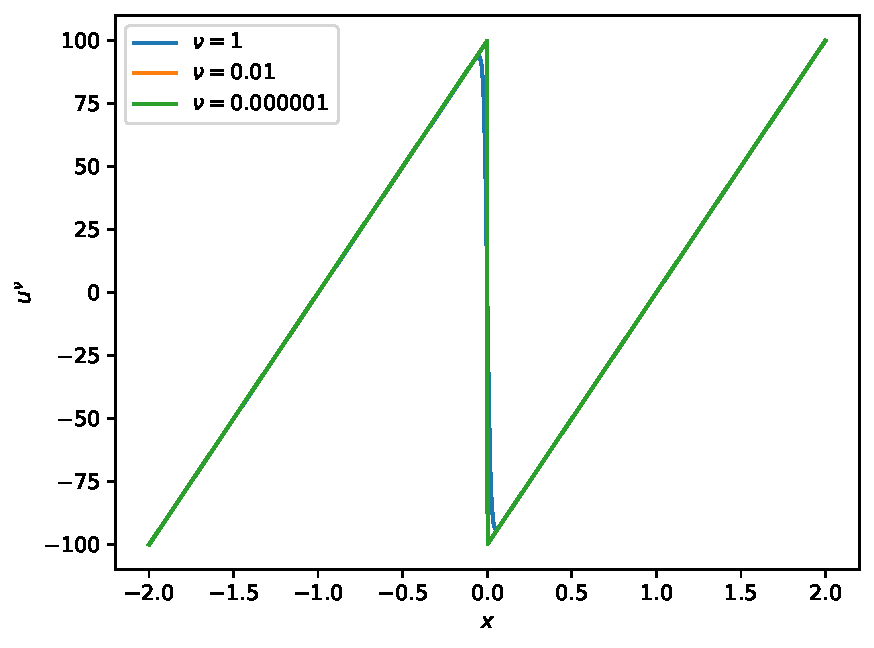
\includegraphics[width=\textwidth]{Images/burger_t=0.01.pdf}
              \caption{$t = 0.01$}
            \end{subfigure}
            \begin{subfigure}{0.32\textwidth}
              \centering
              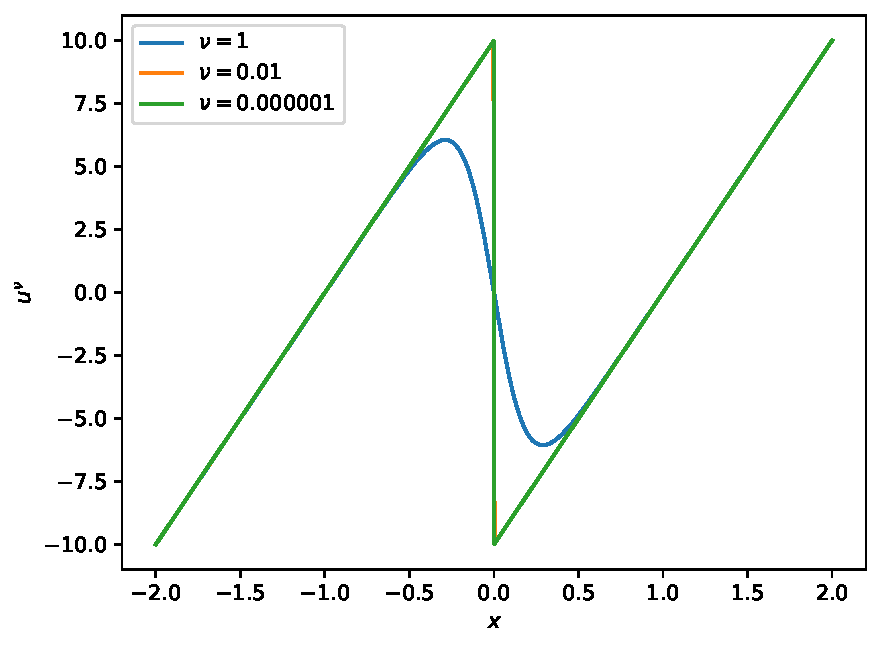
\includegraphics[width=\textwidth]{Images/burger_t=0.1.pdf}
              \caption{$t = 0.1$}
            \end{subfigure}
            \begin{subfigure}{0.32\textwidth}
              \centering
              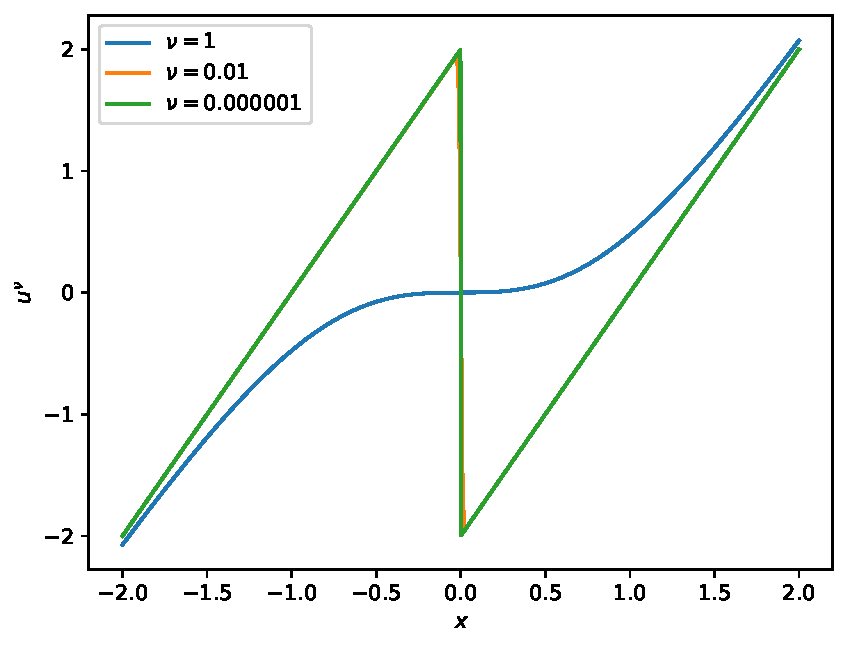
\includegraphics[width=\textwidth]{Images/burger_t=0.5.pdf}
              \caption{$t = 0.5$}
            \end{subfigure}\\
            \begin{subfigure}{0.32\textwidth}
              \centering
              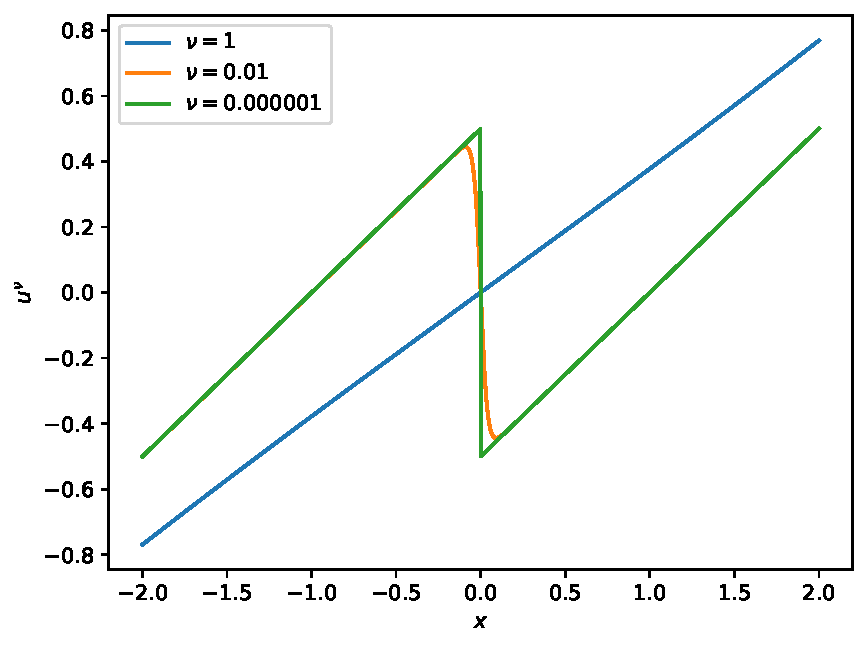
\includegraphics[width=\textwidth]{Images/burger_t=2.pdf}
              \caption{$t = 2$}
            \end{subfigure}
            \begin{subfigure}{0.32\textwidth}
              \centering
              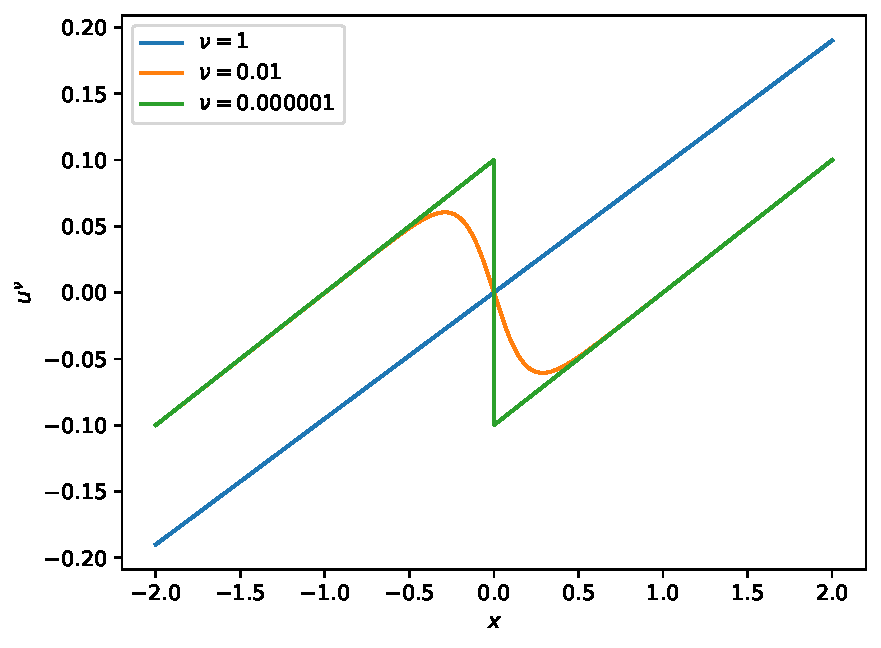
\includegraphics[width=\textwidth]{Images/burger_t=10.pdf}
              \caption{$t = 10$}
            \end{subfigure}
            \begin{subfigure}{0.32\textwidth}
              \centering
              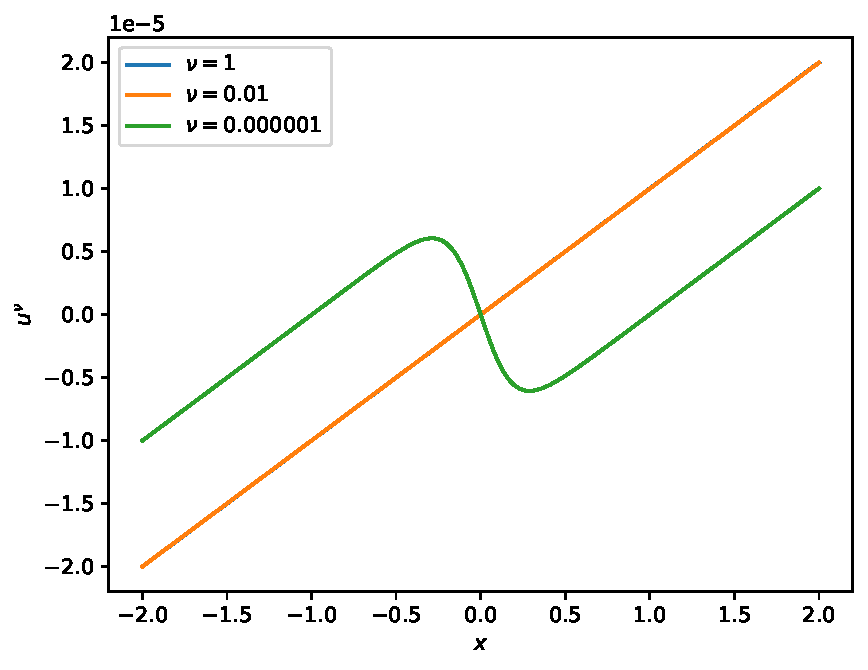
\includegraphics[width=\textwidth]{Images/burger_t=100000.pdf}
              \caption{$t = 10^5$}
            \end{subfigure}
            \caption{Khokhlov velocity field for different values of $t$ and $\nu$.}
            \label{fig:1}
          \end{figure}
    \item Fix $x\in\RR$ and $t>0$. Then, since $\displaystyle \lim_{y\to\pm\infty} \tanh(y) = \pm 1$, we have that:
          \begin{equation*}
            u(x,t):=\lim_{\nu\to 0} u^\nu(x,t) = \lim_{\nu\to 0} \frac{x - L \tanh(Lx/(2\nu t))}{t} =  \frac{\displaystyle x - L \lim_{\nu\to 0} \tanh(Lx/(2\nu t))}{t} = \frac{x - L\sign(x)}{t}.
          \end{equation*}
          Which is not continuous at $x = 0$ for any $t>0$. This is the signature of a shock.
  \end{enumerate}
\end{res}
\begin{exercici}
  The Hopf-Cole transformation is defined as:
  \begin{equation}
    V_i = -2\nu \partial_i \log(\Phi).\label{eq:21}
  \end{equation}
  \begin{enumerate}
    \item Find the link between $\Psi$ and $\Phi$.
    \item Show that the equation for $\Phi$ is linear. It is called the heat equation, that has the interesting property of having simple solutions.
    \item Consider the 1D Case. Find a solution of the heat equation in case of periodic boundary conditions. (Trick: use Fourier transform).
  \end{enumerate}
\end{exercici}
\begin{res}\hfill
  \begin{enumerate}
    \item For each $i$, we have that $-\partial_i \Psi = -2\nu \partial_i\log(\Phi)$. Thus, integrating with respect to $x_i$ we get $\Psi = 2\nu \log(\Phi) + g(t)$, and again the constant $g(t)$ does not depend on any spatial variable $i$ (by the same argument as in \cref{ex:1}). We can in fact determine $g$ from \cref{eq:psi}. Since $V_i=-\partial_i(2\nu \log(\Phi))$, then by \cref{ex:1}, $2\nu \log \Phi$ satisfies also \cref{eq:psi} and thus by the linearity of the derivatives, we get that $g'(t) = f(t)$.
    \item From \cref{eq:psi} we get:
          \begin{align*}
            \partial_t \Psi - \frac{1}{2}(\partial_j \Psi)^2                               & = \nu \laplacian  \Psi + f(t)                                                                   \\
            \partial_t (2\nu\log(\Phi) + g(t)) - \frac{1}{2}(2\nu \partial_j \log(\Phi))^2 & = \nu \laplacian  (2\nu \log(\Phi)) + f(t)                                                      \\
            \frac{\partial_t\Phi}{\Phi} -\nu \left(\frac{\partial_j\Phi}{\Phi}\right)^2    & = \nu \left(\frac{\partial_j^2\Phi}{\Phi} - {\left(\frac{\partial_j\Phi}{\Phi}\right)}^2\right) \\
            \partial_t\Phi                                                                 & = \nu \laplacian \Phi
          \end{align*}
          And this equation is linear in $\Phi$.
    \item The 1D heat equation is $\partial_t \Phi = \nu \partial_{xx} \Phi$. We assume it is defined in a domain $[-L/2,L/2]$, and we equip it with periodic boundary conditions. Now we express the solution in Fourier series $$\Phi(x,t) = \sum_{n\in\ZZ} \widehat{\Phi}_n(t) \exp{\frac{2\pi\ii nx}{L}}$$
          Plugging this formula into the equation we get:
          \begin{equation*}
            \partial_t \widehat{\Phi}_n= -\nu \left(\frac{2\pi n}{L}\right)^2 \widehat{\Phi}_n
          \end{equation*}

          This is a linear ode, whose solution is $\widehat{\Phi}_n(t) = \widehat{\Phi}_n(0) \exp{-\nu \left(\frac{2\pi n}{L}\right)^2 t}$. Thus, the solution $\Phi(x,t)$ is:
          \begin{equation*}
            \Phi(x,t) = \sum_{n\in\ZZ} \widehat{\Phi}_n(0) \exp{\frac{2\pi\ii nx}{L}} \exp{-\nu \left(\frac{2\pi n}{L}\right)^2 t}
          \end{equation*}
  \end{enumerate}
\end{res}
\begin{exercici}
  At very large scale, the Universe is described by Newton equations in a flat, expanding geometry. The equations are:
  \begin{align}
    \partial_t u_i + \frac{\dot{a}}{a} u_i + \frac{1}{a} u_j \partial_j u_i      & = -\frac{1}{a} \partial_i \Phi,\label{eq:31} \\
    \partial_t \rho + 3 \frac{\dot{a}}{a} \rho + \frac{1}{a} \partial_j \rho u_j & = 0,\label{eq:32}                            \\
    \laplacian \Phi                                                              & = 4\pi G a^2 (\rho - \rho_b),\label{eq:33}
  \end{align}
  where $a(t)$ is the expansion factor, $\Phi$ is the gravitational potential, $\rho$ is the density and $u$ is the velocity of the gas. Show that these equations can be mapped into inviscid Burgers equation ($\nu = 0$) by using Zeldovich transformation:
  \begin{align}
    V                                                                      & = \frac{u}{a\dot{b} } = -\nabla \tilde{\Psi} \\
    \label{eq:b}\left(\partial_t + 2 \frac{\dot{a}}{a}\right) \partial_t b & = 4\pi G \rho_b(t)b                          \\
    \tilde{\Phi}                                                           & = \frac{\Phi}{4\pi G \rho_b a^2 b}           \\
    \tilde{\Phi}                                                           & = \tilde{\Psi}
  \end{align}
\end{exercici}
\begin{res}
  We have that $u_i=-a\dot{b} \partial_i \tilde{\Psi}$. Then, introducing this into \cref{eq:31} we get:
  \begin{align*}
    \partial_t u_i + \frac{\dot{a}}{a} u_i + \frac{1}{a} u_j \partial_j u_i                                                                                                                                                            & = -\frac{1}{a} \partial_i \Phi               \\
    -\dot{a} \dot{b} \partial_i\tilde{\Psi} -a\ddot{b} \partial_i\tilde{\Psi} -a\dot{b} \partial_i\partial_t \tilde{\Psi} - \dot{a} \dot{b} \partial_i\tilde{\Psi} -a\dot{b}^2 \partial_j\tilde{\Psi} \partial_j\partial_i\tilde{\Psi} & = -4\pi G \rho_b a b \partial_i\tilde{\Psi}  \\
    -a\dot{b} \partial_i\partial_t \tilde{\Psi} -4\pi G \rho_b a b \partial_i\tilde{\Psi} -a\dot{b}^2 \partial_j\tilde{\Psi} \partial_j\partial_i\tilde{\Psi}                                                                          & = - 4\pi G \rho_b a b \partial_i\tilde{\Psi} \\
    -a\dot{b} \partial_i\partial_t \tilde{\Psi} -a\dot{b}^2 \partial_j\tilde{\Psi} \partial_j\partial_i\tilde{\Psi}                                                                                                                    & = 0
  \end{align*}


  % We take $V_i=\frac{u_i}{a\dot{b}}$, where $b$ satisfies \cref{eq:b}. Then, we have:
  % \begin{align*}
  %   \partial_t V_i + V_j \partial_j V_i & = \frac{1}{a\dot{b}} \partial_t u_i - \frac{u_i}{a^2\dot{b}^2}(\dot{a}\dot{b}+a\ddot{b}) + \frac{1}{a^2\dot{b}^2} u_j \partial_j u_i           \\
  %                                       & = \frac{1}{a\dot{b}} \partial_t u_i - \frac{u_i}{a^2\dot{b}^2}(4\pi G \rho_b a b - \dot{a}\dot{b}) + \frac{1}{a^2\dot{b}^2} u_j \partial_j u_i \\
  %                                       & = \frac{1}{a\dot{b}} \left[ \partial_t u_i +\frac{\dot{a}}{a}u_i+...\right]
  % \end{align*}
  % Moreover, we have that:
  % \begin{align*}
  %   -\partial_i \tilde{\Psi} & = -\partial_i \left(\frac{\Phi}{4\pi G \rho_b a^2 b}\right)                                              \\
  %                            & = -\frac{1}{4\pi G \rho_b a^2 b} \partial_i \Phi - \frac{\Phi}{4\pi G \rho_b a^2 b^2} \grad b            \\
  %                            & = -\frac{1}{4\pi G \rho_b a^2 b} \grad \Phi - \frac{1}{4\pi G \rho_b a^2 b} \grad b = \frac{u}{a\dot{b}}
  % \end{align*}
\end{res}
\begin{exercici}
  Burgers equation develop finite time singularities. Let us study this in the 1D case.
  \begin{enumerate}
    \item\label{ex4:a} Use \eqref{eq:12} to write an equation for $A = \partial_x u$.
    \item Introduce the Lagrangian derivative $D_t A = \partial_t A + u\partial_x A$. Use \ref{ex4:a} to find the ordinary differential equation that links $A$ and its Lagrangian derivative.
    \item Integrate this equation in the case $\nu = 0$, and discuss in which condition there is a finite time blow up of $A$.
    \item Use this discussion to explain the features of the Khokhlov solution at $\nu \to 0$ (presence of positive ramps and no negative ramps).
    \item BONUS question: Can this method be used to study potential blow-up in Euler equation?
  \end{enumerate}
\end{exercici}
\begin{res}\hfill
  \begin{enumerate}
    \item Taking $\partial_x$ to the 1D Burgers equation $\partial_t u + u\partial_x u = \nu \partial_{xx} u$, we get:
          \begin{equation*}
            \partial_t \partial_x u + \partial_x(u\partial_x u) = \nu \partial_{xxx} u
          \end{equation*}
          Thus:
          \begin{equation}\label{eq:A}
            \partial_t A + u\partial_x A + A^2 = \nu \partial_{xx} A
          \end{equation}
    \item From \cref{eq:A} we get:
          \begin{equation*}
            D_t A + A^2 = \nu \partial_{xx} A
          \end{equation*}
    \item For $\nu=0$ we have:
          \begin{equation*}
            D_t A + A^2 = 0
          \end{equation*}
          Separating variables we get:
          \begin{equation*}
            \frac{dA}{A^2} = -dt
          \end{equation*}
          Integrating between $s=t_0$ and $s=t$ we get:
          \begin{equation*}
            \frac{1}{A(t,x(t))} - \frac{1}{A(t_0,x(t_0))} = t-t_0
          \end{equation*}
          Thus:
          \begin{equation*}
            A(t,x(t)) = \frac{A(t_0,x(t_0))}{1+A(t_0,x(t_0))(t-t_0)}
          \end{equation*}
          We have a finite time blow up of $A$ at $t=t_0-1/A(t_0,x(t_0))$.
    \item We take $t_0=0$
    \item
  \end{enumerate}
\end{res}
\end{document}


